% !TEX root = ../main.tex
\subsection{RG-E Experiment}
\label{11.300::rge_experiment}
    The RG-E experiment, to be conducted in Hall B, focuses on measuring the hadronic multiplicity ratio between various nuclei and deuterium.
    To achieve this, a double-target system is being constructed.
    This system will enable a precise comparison between a deuterium target and heavy solid targets such as carbon, aluminium, copper, tin, lead, and others.
    The primary objective of the experiment is to enhance our understanding of hadronisation in the nuclear medium, colour transparency, and nuclear short-range correlations.

    During the data acquisition process, both the cryo-target (deuterium) and a solid target will be exposed to the electron beam simultaneously.
    To minimize differences in acceptance corrections between the targets, efforts are made to maintain a minimal distance between them.
    However, it is crucial to ensure that the targets can still be differentiated during the reconstruction process.
    The work behind this thesis contributes to the experiment by improving the offline reconstruction methods prior to the actual experiment, with the aim of reducing the distance between the targets.
    Further details on this topic can be found in Section \ref{12::fmt_alignment_and_reconstruction}.

    Simultaneously positioning both targets in the beam allows for the cancellation of time-dependent systematic effects, thereby increasing the precision of the final results.
    These effects can include drifting gains and inefficient detector channels when measuring ratio-like observables.
    Since the target system will be placed in a vacuum, the switching between solid targets needs to be done remotely.
    It is essential to perform the switching quickly to maximise the beam time available for the experiment.

    The double target system is designed to enable switching between up to five different solid targets.
    Previous experiments, such as EG2 conducted on the former CLAS, have demonstrated that the design of the double target system offers significant advantages in reducing systematic uncertainties \cite{hakobyan2008}.
    The principle of the target system involves installing the solid targets on a carbon fibre band that slides on torlon rails.
    The movement of the band is accomplished using a piezo-motor, chosen for its insensitivity to magnetic fields.
    Figure \ref{fig::11.300::double_target} illustrates the proposed design of the double target system.

    \begin{figure}[b!]
        \frame{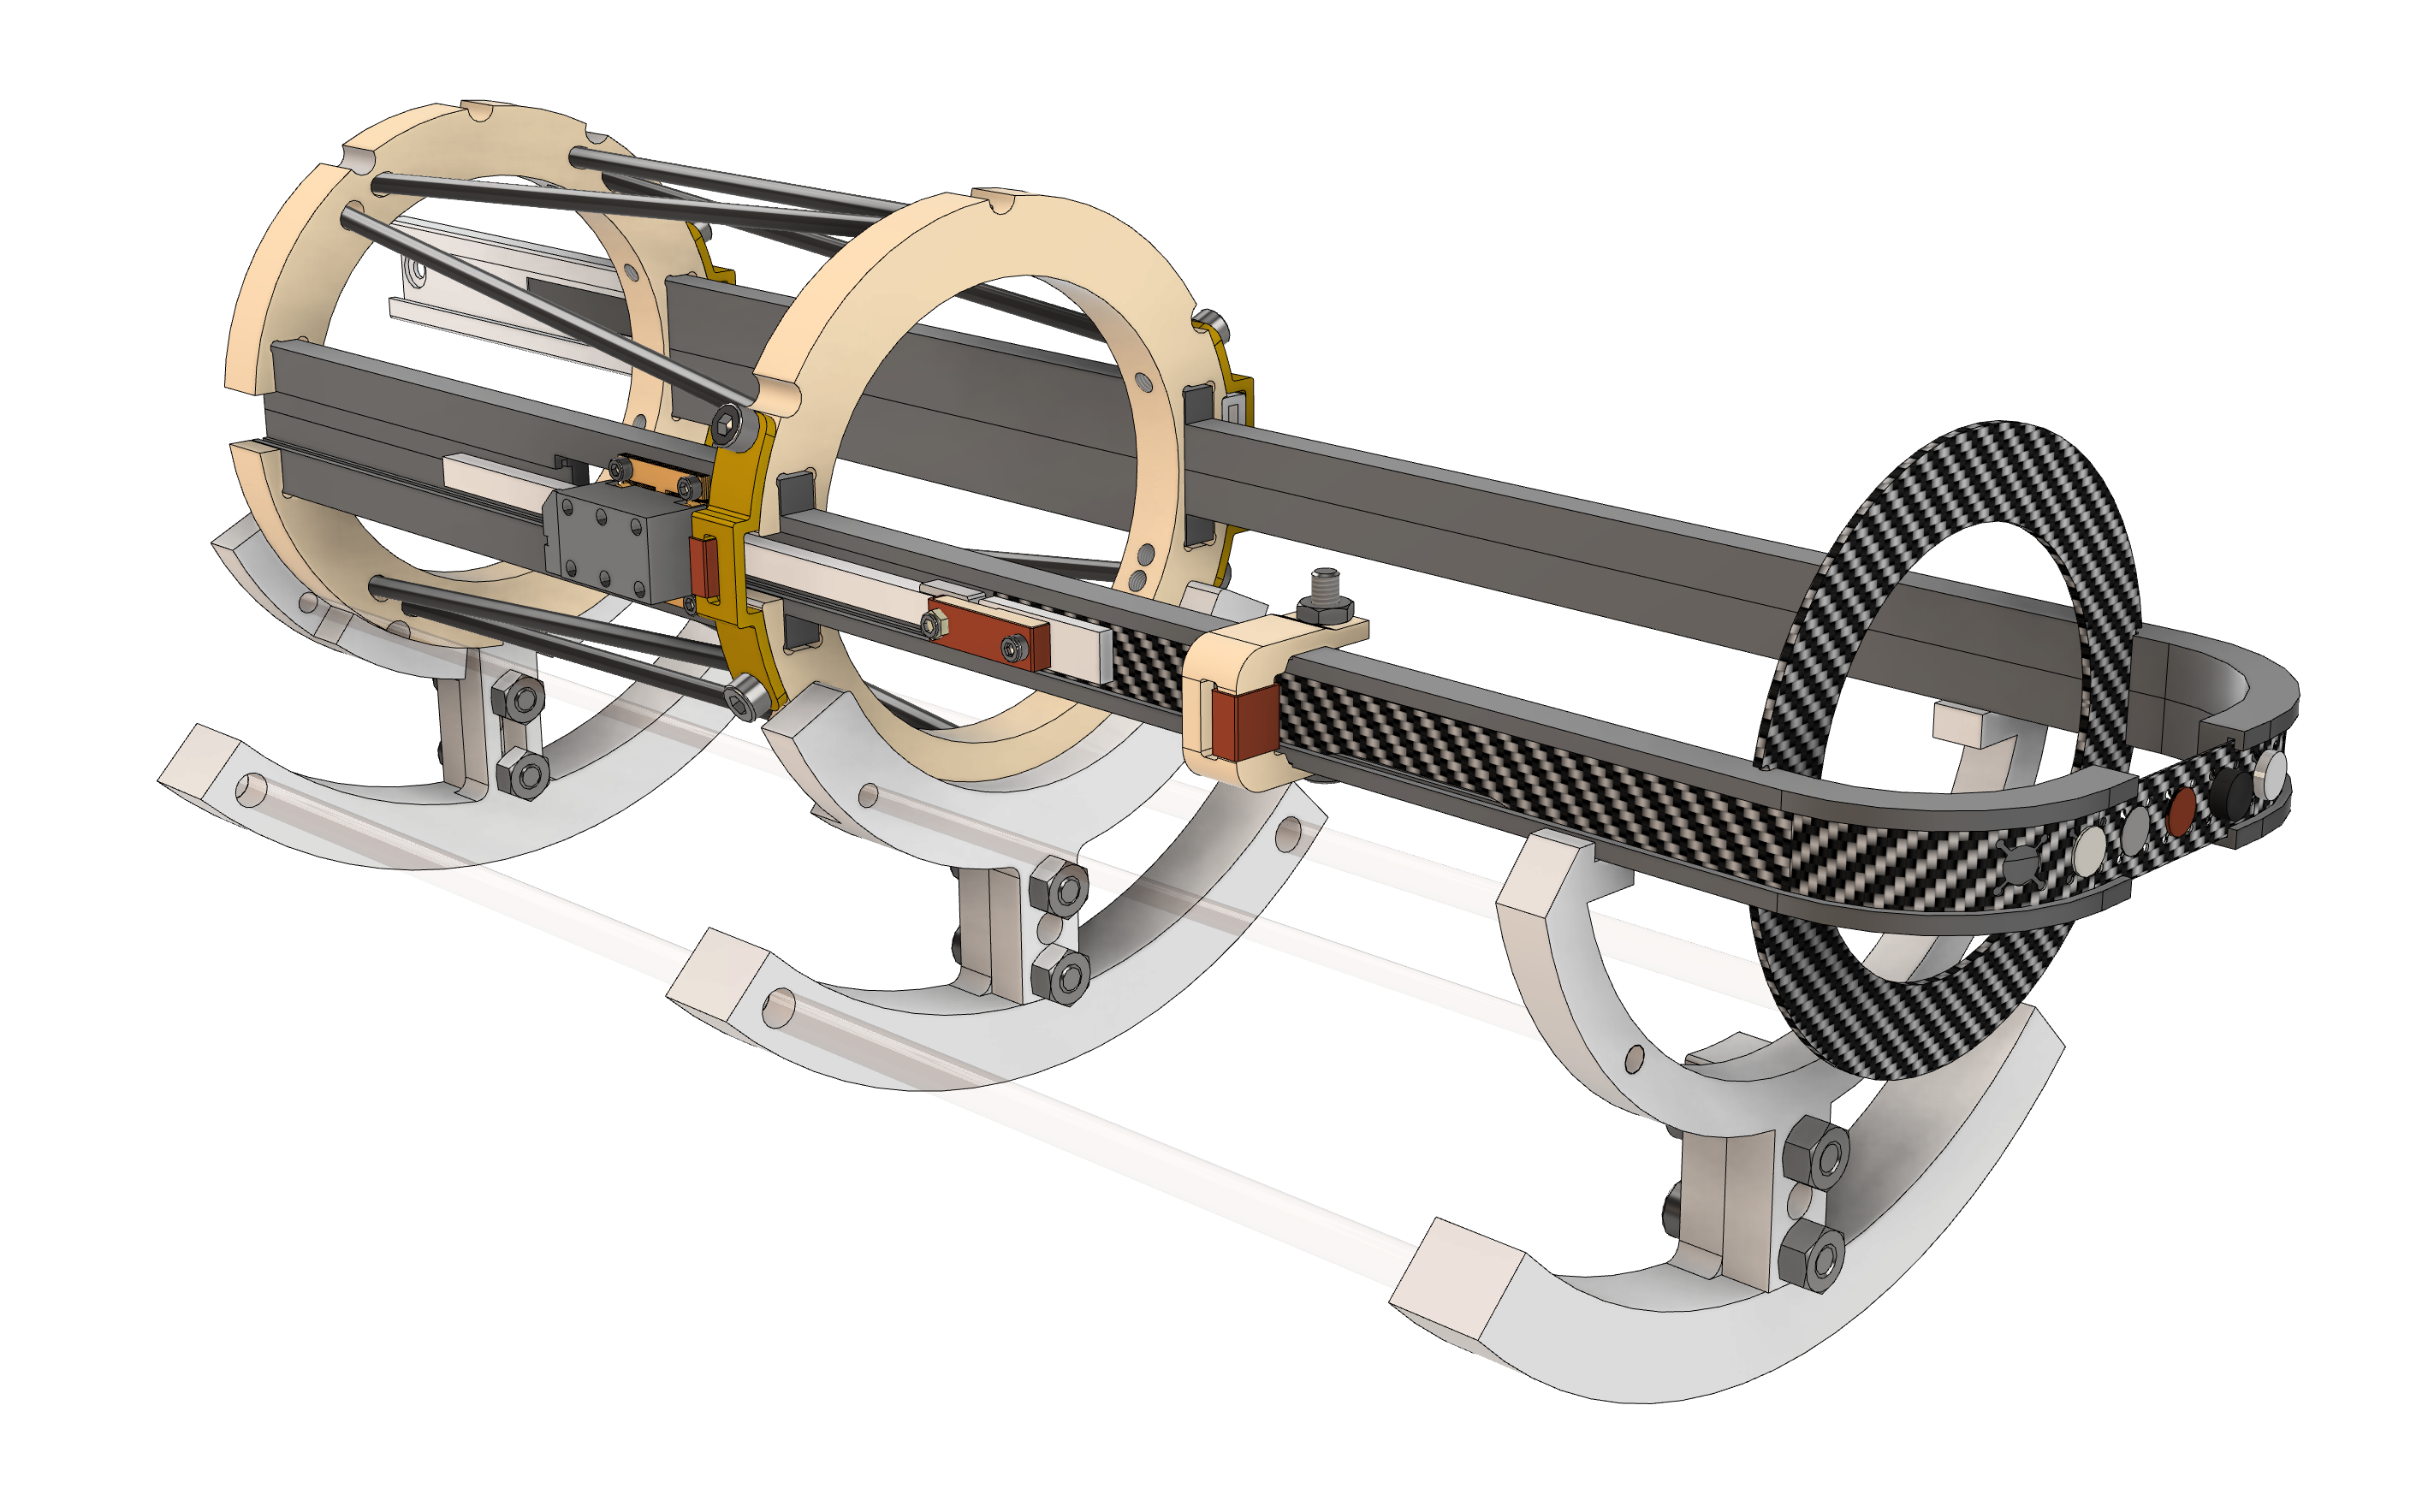
\includegraphics[width=\textwidth]{300double_target.png}}
        \caption[Double-target system.]
        {Double-target system CAD render.}
        \floatfoot{Source: Render by Alonso Lepe, from the Double Target group.}
        \label{fig::11.300::double_target}
    \end{figure}

    To ensure the proper functioning of the target, a series of tests have been conducted.
    These tests cover various aspects of the target's operation and performance.
    They include:

    \begin{itemize}
        \item
            Movement under vacuum and high magnetic field:
            The target system has been tested to ensure that it can operate smoothly and reliably under vacuum conditions and in the presence of high magnetic fields.
            This is important to verify that the target's movement and positioning are not affected by these conditions.

        \item
            Radiation hardness of selected materials:
            The materials used in the target system have been tested for their resistance to radiation.
            This is crucial because the target may be exposed to radiation during the experiment.
            By assessing the radiation hardness of the materials, it can be ensured that they will maintain their structural integrity and functionality throughout the experiment.

        \item
            Heat removal tests:
            The target system has undergone heat removal tests to ensure that it can effectively dissipate heat generated during operation.
            It is essential to keep the target temperature well below its melting point to prevent any damage or degradation.
            By conducting heat removal tests, the target's cooling capabilities have been evaluated to ensure optimal performance and longevity.
    \end{itemize}

    These tests collectively aim to validate the target's operational robustness and reliability under the specific conditions of the experiment, thereby ensuring accurate and consistent data collection.

    % !TEX root = ../main.tex
\subsubsection{Slow Control System}
\label{sssec::slow_control_system}
% --+ What is slow control +----------------------------------------------------
    A modern experimental physics experiment usually involves many moving parts and complex components that require constant monitoring and calibration.
    Additionally, continuous data collection is necessary.
    This task is accomplished through the use of slow control systems.
    These systems typically integrate the entire detector and experiment into one complex interface, facilitating easy access and maintenance.

% --+ What is EPICS +-----------------------------------------------------------
    The standard framework used in the context of HEP for achieving this is the Experimental Physics and Industrial Control System (EPICS).
    EPICS was developed at the Los Alamos National Laboratory (ANL) to facilitate data acquisition and control for such experiments.
    This framework offers a distributed process control system that includes software communication, functional subsystems for data acquisition, supervisory control, closed-loop control, channel archiving, and alarm management \cite{dalesio1991}.

    Similar to many HEP experiments, the slow control system of CLAS12 is based on EPICS \cite{boyarinov2020}.

% --+ EPICS installation on raspi +---------------------------------------------
    To enable the integration of the RG-E target into the CLAS12 slow control system, the author developed an EPICS support module and Input/Output Controller (IOC).
    This module was not created from scratch since the motor developers had already developed a generic support module for Galil motors \cite{farnswort2009}.
    The existing system proved to be capable of supporting the movement of the RG-E target system, requiring only the removal of unnecessary features and the addition of experiment-specific database variables.

    The RG-E IOC, along with the complete set of EPICS support modules necessary to run it, can be found at

    \begin{center}
        \hyperlink{https://github.com/bleaktwig/rge-epics-support}{\texttt{https://github.com/bleaktwig/rge-epics-support}}.
    \end{center}

    The EPICS module includes Process Variables (PVs) that have been added to facilitate the control of the RG-E target system.
    Below is a list of these PVs along with a brief description of each.
    The user-defined records database, where these PVs can be viewed and edited, is located at

    \begin{center}
        \texttt{\$EPICS\_BASE/support/galil/3-6/db/galil\_userdef\_records.template}.
    \end{center}

    % !TEX root = ../main.tex
% --+ ai +----------------------------------------------------------------------
\paragraph{Analog Input (\texttt{ai})}
    The normal use for this record type is to obtain an analog value from hardware and then convert it to engineering units \cite{stanley1998}.
    The record can also be used to write constants to be read from the database, such that they can be changed in runtime.

    \subparagraph{\texttt{DMC01:A\_curr\_pos}.}
        Current position of the band.
        Displayed at the Graphical User Interface (GUI) and used for internal calculations.

    \subparagraph{\texttt{DMC01:A\_home}.}
        Position of the home.
        Displayed at the GUI and used for calculations.

    \subparagraph{\texttt{DMC01:A\_pos\#}.}
        \# is a number from 1 to 7.
        Positions of each of the seven targets.
        Displayed at the GUI and used for calculations.

    \subparagraph{\texttt{DMC01:A\_lowlimit}.}
        Position of the low limit.
        If \texttt{DMC01:A\_curr\_pos} is lesser than this value, a major alarm is fired.

    \subparagraph{\texttt{DMC01:A\_highlimit}.}
        Position of the high limit.
        If \texttt{DMC01:A\_curr\_pos} is greater than this value, a major alarm is fired.

    \subparagraph{\texttt{DMC01:A\_tolerance}.}
        Equivalence tolerance for the position of each target and the position of the band.
        It defines a valid range around the target position.

    \subparagraph{\texttt{DMC01:COMMERR\_STATUS}.}
        Variable that is true when there's a communication error with the controller and false otherwise.
        Used for triggering a communication alarm.

    \subparagraph{\texttt{IOC01:SR\_i\_am\_alive}.}
        Variable that is true when the IOC is up and running, false otherwise.
        Used for triggering a communication alarm.

% --+ ao +----------------------------------------------------------------------
\paragraph{Analog Output (\texttt{ao})}
    The normal use for this record type is to output values to digital-analog converters.
    The desired output can be controlled by either an operator or a state program, or it can be fetched from another record \cite{stanley1998}.

    \subparagraph{\texttt{DMC01:A\_go\_home}.}
        Command to move the band to the home position, as defined in \texttt{DMC01:A\_home}.

    \subparagraph{\texttt{DMC01:A\_go\_pos\#}.}
        Command to move the band to the position of target \#, as defined in \texttt{DMC01:A\_pos\#}.

% --+ calc +--------------------------------------------------------------------
\paragraph{Calculation (\texttt{calc})}
    The calculation or ``Calc'' record is used to perform algebraic, relational, and logical operations on values retrieved from other records.
    The result of its operations can then be accessed by another record so that it can be used \cite{stanley1998}.
    In the context of the RG-E target, each calculation returns a number from 0 to 11.
    This number represent the state the target is in, and is later used by a Select PV.

    \subparagraph{\texttt{DMC01:A\_at\_pos\#}.}
        Calculation that checks if the band position is equal to that of target \# in \texttt{DMC01:A\_pos\#}, within the tolerance margin \texttt{DMC01:A\_tolerance}.
        If it is, it returns \#.
        Otherwise, it returns 0.

    \subparagraph{\texttt{DMC01:A\_at\_home}.}
        Calculation that checks if the band position is equal to the home position in \texttt{DMC01:A\_home}, within the tolerance margin defined by the tolerance.
        If it is, it returns 8.
        Otherwise, it returns 0.

    \subparagraph{\texttt{DMC01:A\_moving}.}
        Calculation that checks if the target is moving by checking the motor PV \texttt{DMC01:A.MOVN}.
        If it is, it returns 9.
        Otherwise, it returns 0.

    \subparagraph{\texttt{DMC01:A\_at\_lowlimit}.}
        Calculation that checks if the band position is lesser than the low limit \texttt{DMC01:A\_lowlimit}.
        If it is, it returns 10.
        Otherwise, it returns 0.

    \subparagraph{\texttt{DMC01:A\_at\_highlimit}.}
        Calculation that checks if the band position is greater than the high limit \texttt{DMC01:A\_highlimit}.
        If it is, it returns 11.
        Otherwise, it returns 0.

% --+ sel +---------------------------------------------------------------------
\paragraph{Select (\texttt{sel})}
    The select record computes a value based on input obtained from up to 12 locations \cite{stanley1998}.
    By default, it is equal to the highest value among its input PVs.

    \subparagraph{\texttt{DMC01:A\_sel\_tgttype}.}
        This record returns the highest value between the previously defined calculations.
        Thus, it associates the values returned to a state of the target.
        By convention, this PV assumes that \emph{no more than one \texttt{calc} is greater than 0}.
        This assumptions holds as long as \texttt{DMC01:A\_tolerance} is not set higher than half the distance between targets and between the targets and the lower and higher limits.

% --+ mbbi +--------------------------------------------------------------------
\paragraph{Multi-Bit Binary Input (\texttt{mbbi})}
    The normal use for the multi-bit binary input record is to read multiple bit inputs from hardware.
    The binary value represents a state from a range of up to 16 states.
    The multi-bit input record interfaces with devices that use more than one bit \cite{stanley1998}.

    \subparagraph{\texttt{DMC01:A\_tgttype}.}
        This \texttt{mbbi} encodes the output of \texttt{DMC01:A\_sel\_tgttype} to a string and alarm level.
        The encoding is specified in Table \ref{tab::11.311::target_type_pv}.

% --+ Everything table +--------------------------------------------------------
\begin{table}[b!]
    \begin{center}
        \begin{tabularx}{220pt}{lll}
            \toprule
            \textbf{Value} & \textbf{Name} & \textbf{Alarm Severity} \\
            \midrule \midrule
             0             & Not Moving    & Major          \\
             1             & Target 1      & No alarm       \\
             2             & Target 2      & No alarm       \\
             3             & Target 3      & No alarm       \\
             4             & Target 4      & No alarm       \\
             5             & Target 5      & No alarm       \\
             6             & Target 6      & No alarm       \\
             7             & Target 7      & No alarm       \\
             8             & Home          & No alarm       \\
             9             & Moving        & Minor          \\
            10             & Low Limit     & Major          \\
            11             & High Limit    & Major          \\
            \bottomrule
        \end{tabularx}
    \end{center}

    \caption{Names and alarm levels for the different values of the PV \texttt{DMC01:A\_tgttype}.}
    \label{tab::11.311::target_type_pv}
\end{table}

    % !TEX root = ../main.tex
\paragraph{CS-Studio}
    The Graphical User Interface (GUI) of CLAS12 EPICS is built on the Control System Studio (CS-Studio) toolkit.
    CS-Studio is specifically designed for monitoring and operating large-scale control systems and is based on the eclipse Rich Client Platform (RCP) framework \cite{kasemir2007}.
    To integrate the RG-E target system into CLAS12 EPICS, a CS-Studio screen was developed.

    Below is a list of the requirements that the screen needed to fulfil.
    These requirements were derived from the specifications of the physics experiments as well as the needs of the electronics team responsible for the target system.

    \begin{itemize}
        \item
            Buttons to move the target band to the targets and a home location.
        \item
            A Button to stop the target band in case of emergency.
        \item
            A status check on the position of the target band.
        \item
            Alarm handling for the case when the band moves beyond low and high limits.
        \item
            Alarm handling for the IOC and communication problems.
    \end{itemize}

    \begin{figure}[b!]
        \centering\frame{
        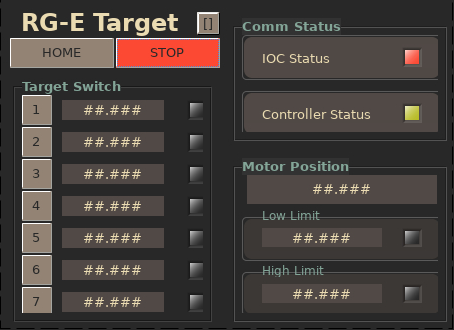
\includegraphics[]{312motorx_rge.png}}
        \caption[RG-E CS-Studio main screen]{RG-E CS-Studio main screen. The HOME and A, B, C, etc buttons move the target strip to the corresponding location, the STOP button is an emergency, instant stop of the target system, and the Motor Screens button allows the user to open additional motor screens.
        Source: Own Elaboration using \hyperlink{controlsystemstudio.org/}{CS-Studio}.}
        \label{fig::11.312::rge_motorx}
    \end{figure}

The implemented screen, shown in Figure \ref{fig::11.312::rge_motorx}, incorporates these requirements.
    Along with the buttons, text displays indicate the position of each target within the band.
    Adjacent LED displays illuminate green when the band position aligns with the target position, within the tolerance specified in the database.
    Additionally, four LED displays are positioned to the right of the two IOC statuses, as well as the low and high limits.
    These LEDs indicate alarm conditions and work in conjunction with the CLAS12 Slow Control alarm system to alert the user of any issues.

    Furthermore, in addition to the aforementioned screen, users can access other screens through the Motor Screens menu button.
    These screens are part of the motor EPICS support module and are retained for debugging purposes.
    They include a manual motor movement screen, a motor setup screen, a direct Command Line Interface (CLI) with the motor, and an amplifier configuration screen.
    All of these screens were developed by the Galil EPICS team \cite{farnswort2009}.

    To enhance user experience, the GUI was designed using the Gruvbox colour palette.
    This palette is specifically chosen to ensure that colours are easily distinguishable, with sufficient contrast, while also being visually appealing and comfortable for the eyes.
    The Gruvbox colour palette can be found on GitHub at

    \begin{center}
        \hyperlink{github.com/morhetz/gruvbox}{\texttt{github.com/morhetz/gruvbox}}.
    \end{center}

    % !TEX root = ../main.tex
\paragraph{Alarm System}
\label{par::alarm_system}
    To ensure the reliable operation of the CLAS12 detector, all EPICS-controlled subsystems within it are equipped with PVs that define alarm conditions.
    These alarms, along with their severity, associated subsystems, and pre-defined instructions on how to respond to them, are displayed in a centralised alarm system.

    For each experiment conducted in Hall B involving a non-trivial target system, a specific set of alarms is required.
    In the case of the RG-E target, the list of implemented alarms and their corresponding PVs is provided in Table \ref{tab::alarms_pv}.

    \begin{table}[b!]
        \caption{Alarm names, triggers, and severities for the RG-E target slow control system.}

        \begin{center}
            \begin{tabularx}{360pt}{llX}
                \hline
                \textbf{Name}          & \textbf{Trigger}                     & \textbf{Severity} \\
                \hline
                Band is not moving     & \texttt{DMC01:A\_tgttype}       =  0 & Major             \\
                Band is moving         & \texttt{DMC01:A\_tgttype}       =  9 & Minor             \\
                Band beyond low limit  & \texttt{DMC01:A\_tgttype}       = 10 & Major             \\
                Band beyond high limit & \texttt{DMC01:A\_tgttype}       = 11 & Major             \\
                Controller comm. error & \texttt{DMC01:COMMERR\_STATUS}  =  1 & Major             \\
                IOC comm. error        & \texttt{IOC01:SR\_i\_am\_alive} =  0 & Major             \\
                \hline
            \end{tabularx}
            \label{tab::alarms_pv}
        \end{center}
    \end{table}


